\chapter{Statistical Fit} \label{chap:fit}

The final significance of $V$ + jets and Higgs + jets production are quantified
through a Bayesian implementation of a likelihood function.  This procedure
uses the information known about the systematic uncertanties and normalization
of the signal before the fit, called priors, along with the template histograms
representing the impact of each prior on the distribution of interest $m_{J}$.
These priors are then iteratively updated by the data, contained in a
likelihood function, using a Markov Chain Monte Carlo procedure.  This results
in a marginalized probability density function (p.d.f) which represents the
probability of there being a number of signal events present in the data.  This
p.d.f is then used to determine the signal strength $\mu_{s}$ and its
uncertainty as well as a 95\% credibility level (CL).  The following chapter
will discuss the theory and implementation of these ideas in the context of the
systematics presented in \Cref{chap:systematics} using the Bayesian Analysis
Toolkit (BAT) \cite{Beaujean:2011zz}.

\section{Limit Setting and Bayes' Theorem} \label{sec:fit:theory}

\section{Implementation of Priors} \label{sec:fit:priors}

As discussed in \Cref{sec:fit:theory} the priors representing the nuisance
parameters and the signal normalization are chosen to represent the analyzer's
knowledge before the data is considered. Generally speaking, the shape of the
prior distribution for systematic uncertainties is chosen to give decreased
probability as the fit tries to pull the value away from their nominal value,
while for the signal parameter the choice is made to have as little influence
on the marginalized posterior as possible.

For the $t\bar{t}$ signal strength a Gaussian prior is used with the mean and
width determined by the fit to data in the $\text{CR}_{t\bar{t}}$.  The
Gaussian prior is then normalized to unity and defined over the range [$-\nu_{5
\cdot t\bar{t}}, \nu_{5 \cdot t\bar{t}}$], where $\nu_{5 \cdot t\bar{t}}$ is five
times the expected value for $t\bar{t}$, and is set to zero elsewhere.

The remaining nuisance parameters are included using a Gaussian prior for each
source.  The Gaussian for the QCD fit function choice uncertainty is defined in
the range [$0\sigma, 1\sigma$], where $0\sigma$ corresponds to the nominal fit
function and $1\sigma$ corresponds to the alternate fit function.  All other
sources of systematic uncertainty are defined using a Gaussian over the large
range $[-3\sigma, 3\sigma]$ to allow ample room for fluctuations.
 
The two signal models, $V$ + jets and Higgs + jets, are each included in the
combined fit by utilizing a uniform prior to represent the parameter corresponding
to the number of events.  This is done to remove analyzer bias, thus allowing
the final result to more accurately reflect the data.  Furthermore, both priors
are normalized to unity over their respective ranges for reasons discussed in
\Cref{sec:fit:bat}. The $V$ + jets uniform prior is defined to be $1/(2 \cdot
\nu_{5 \cdot V})$ over the range [$-\nu_{5 \cdot V}, \nu_{5 \cdot V}$] and zero
everywhere else. Here $\nu_{5 \cdot V}$ is defined to be five times the expected
value for $V$ + jets. The Higgs + jets uniform prior is defined to be
$1/\nu_{H\text{max}}$ over the range [$0,\nu_{H\text{max}}$] and zero elsewhere.  This
$\nu_{H\text{max}}$ is the number of Higgs + jets events corresponding to the point
where the likelihood is a factor of $10^{5}$ times smaller than its maximum
value.  In both cases the ranges were chosen to be very large so as to not
influence the result.

\section{Bayesian Analysis Toolkit} \label{sec:fit:bat}

The Bayesian Analysis Toolkit (BAT) \cite{Beaujean:2011zz,Beresford:2642397} is
used to obtain the marginalized posterior distribution \Cref{eq:fit:bayes}
discussed in \Cref{sec:fit:theory}.  It takes as input the data, the parameters
$\nu$ and $\boldsymbol{\theta}$ along with their corresponding prior
distributions discussed in \Cref{sec:fit:priors}, and the chosen likelihood
function $\mathcal{L}(\nu,\boldsymbol{\theta}|Data)$.  Here the likelihood
function is given by the product of the Poisson probability in each bin: 

\begin{equation} \label{sec:fit:likelihood}
\mathcal{L}(\nu,\boldsymbol{\theta}|Data) = \prod_{i=1}^{N} \frac{(s_{i}(\nu,\boldsymbol{\theta}) + b_{i}(\nu,\boldsymbol{\theta}))^{n_{i}}}{n_{i}!} e^{-(s_{i}(\nu,\boldsymbol{\theta}) + b_{i}(\nu,\boldsymbol{\theta}))}
\end{equation}

In the above the product runs over all N bins in the histogram being fit,
$s_{i}$ and $b_{i}$ are the expected number of signal and background events
expected in bin $i$ dependant upon $\nu$ and $\boldsymbol{\theta}$, and $n_{i}$
is the number of data events in bin $i$.  Note that in \Cref{sec:fit:priors}
the signal parameter priors are normalized to unity such that $\nu$ corresponds
to the number of signal events. Now \Cref{sec:fit:likelihood} can be used to
calculate the probability of a given set of parameter values $\nu$ and
$\boldsymbol{\theta}$ given the data.  Plugging this definition into
\Cref{eq:fit:bayes} gives us the final form of Bayes' equation used to
calculate the marginalized posterior $p(\nu|\text{Data})$ given below.

\begin{equation} \label{sec:fit:full_bayes}
p(\nu|\text{Data}) \propto \pi(\nu) \int \prod_{i=1}^{N} \frac{(s_{i}(\nu,\boldsymbol{\theta}) + b_{i}(\nu,\boldsymbol{\theta}))^{n_{i}}}{n_{i}!} e^{-(s_{i}(\nu,\boldsymbol{\theta}) + b_{i}(\nu,\boldsymbol{\theta}))} \prod_{j}\pi(\theta_j)\text{d}\boldsymbol{\theta}
\end{equation}

The final step is to calculate the integral in \Cref{sec:fit:full_bayes} across
the multi-dimentional space of $(\nu,\boldsymbol{\theta})$. However, calculating the
integral for such a large space is not computationally feasible so BAT instead
employed a Markov Chain Monte Carlo (MCMC) \cite{Betancourt2017ACI,
Beresford:2642397} in order to sammple the space efficiently.

The basic idea of a MCMC is to perform a random walk in the parameter space
$(\nu,\boldsymbol{\theta})$ making sure to spend more time sampling regions of
high probability, i.ee sampling proportional to the posterior.  The sequence of
parameter values on the walk depends only on the previous set making the
resuling dequence of parameter values a Markov Chain \cite{Markov2006}.  The
Metropolis-Hastings algorithm \cite{10.2307/2334940,Beresford:2642397} is used
to generate the Markov Chains used in BAT.  This procedure is detailed below
and an illustration of the process for only two parameters $\theta_{1}$ and
$\theta_{2}$ is shown in \Cref{sec:fit:markov_chain}.

\begin{enumerate}
\item The chain begins at position $\boldsymbol{x_{1}}$ in the parameter space to be sampled.
\item The next position, $\boldsymbol{x_{2}}$, is proposed by selecting each new parameter from a Breit-Wigner distribution centered on the value of the corresponding parameter for the current position $\boldsymbol{x_{1}}$.
\item A random number $r$ between 0 and 1 is selected from a uniform distribution.
\item The value of the posterior $p(\nu,\boldsymbol{\theta}|\text{Data})$, given in \Cref{eq:fit:posterior}, is calculated for both  $\boldsymbol{x_{1}}$ and  $\boldsymbol{x_{2}}$ resulting in $p(\nu,\boldsymbol{\theta}|\text{Data})_{1}$ and $p(\nu,\boldsymbol{\theta}|\text{Data})_{2}$.
\item If $r < \frac{p(\nu,\boldsymbol{\theta}|\text{Data})_{2}}{p(\nu,\boldsymbol{\theta}|\text{Data})_{1}}$, the algorithm transitions to the new position $\boldsymbol{x_{2}}$ and it is added to the chain. Otherwise the algorithm remains at $\boldsymbol{x_{1}}$ and it is added to the chain.
\item This process is then repeated starting from the chosen position defined as position $\boldsymbol{x_{1}}$.
\end{enumerate}

\begin{figure}[!htbp]
\centering
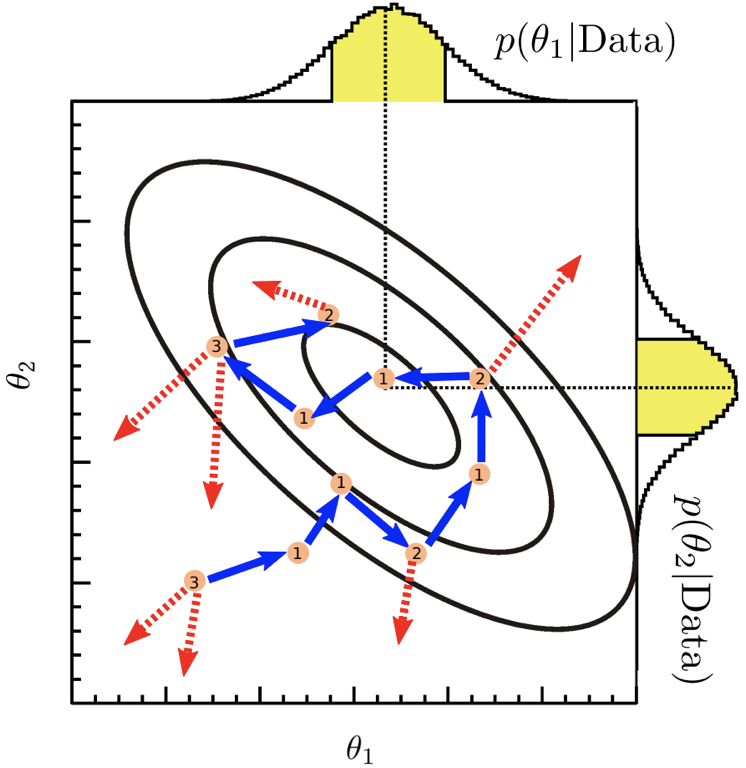
\includegraphics[width=0.7\linewidth]{figures/fit/markov_chain}
\caption{\cite{Beresford:2642397}This figure illustrates a random walk in parameter space $(\theta_{1},\theta{2})$. The numbers indicate the number of iterations the chain remained at this point in parameter space, the blue arrows indicate accepted transitions, and the red arrows indicate rejected transitions. The marginalised posterior distributions obtained for the two parameters $p(\theta_{1}|Data)$ and $p(\theta_{2}|Data)$ are also shown, and the yellow bands correspond to the central 68\% of the distributions.}
\label{sec:fit:markov_chain}
\end{figure}

This random walk in parameter space generates a chain which preferentially
transitions to positions corresponding to high probability regions of the
posterior, effectively sampling the important regions of the posterior
distribution.  By plotting the frequency of occurrence for each parameter along
the chain, and then normalizing the distribution to unity, the desired
marginalized posterior for the signal parameter $p(\nu|\text{Data})$ is found.
In \Cref{chap:results} this marginalized posterior is used to find the final
results of the analysis presented.

